%\documentclass[presentation, smaller, xcolor=table]{beamer}
\documentclass[handout, smaller, xcolor=table]{beamer}			% Suppresses pauses
%\mode<handout>{\setbeamercolor{background canvas}{bg=black!5}}	% very light gray background

\usepackage{pgfpages}
	%\pgfpagesuselayout{resize to}[a4paper, border shrink=5mm, landscape]
	\pgfpagesuselayout{2 on 1}[a4paper, border shrink=5mm]		%[, portrait]
	%\pgfpagesuselayout{4 on 1}[a4paper, border shrink=5mm, landscape]
	
%\setbeameroption{show slides}
%\setbeameroption{show notes}
%\setbeameroption{show only notes}

%%=========================================================================================%%
%% Themes
\usetheme{CambridgeUS}					%AnnArbor, CambridgeUS, Copenhagen, Madrid
\useoutertheme[compress, subsection=false]{miniframes}	%, footline=authorinstitutetitle
\setbeamertemplate{navigation symbols}{}		% Suppress navigation symbols in footer
%\usecolortheme{whale}

\usefonttheme[onlymath]{serif}			% To properly render mathematical symbols
%\usefonttheme[onlylarge]{structurebold}	

\setbeamercolor*{itemize item}{fg=darkred}
\setbeamertemplate{itemize item}[square]
\setbeamercolor*{itemize subitem}{fg=darkred}
\setbeamertemplate{itemize subitem}[circle]
\setbeamercolor*{enumerate item}{fg=darkred}
\setbeamertemplate{enumerate item}[default]

% \usepackage{beamerthemesplit}		% Activate for custom appearance

%\setbeamertemplate{headline}[default]
%\setbeamercolor{footlinecolor}{fg=white,bg=blue}%{whale}%
%\setbeamertemplate{footline}
%{
%	\begin{beamercolorbox}[wd=\paperwidth,ht=4.0ex,dp=1.0ex,leftskip=0cm,rightskip=0cm,sep=1em]{titlelike}
%	\vspace{-2.0ex}
%	\insertshortinstitute
%	\hfill \insertshorttitle
%	\hfill \insertframenumber\,/\,\inserttotalframenumber 
%	%\hspace{0.5cm}
%	\end{beamercolorbox}
%}
%\setbeamertemplate{sidebar right}
%{
%	\vskip10pt \insertshorttitle[width={2.0cm}, center, respectlinebreaks]
%	\vskip10pt \insertshortauthor[width={2.0cm}, center]
%	\vskip10pt \insertshortinstitute[width={2.0cm}, center]
%	\vfill \hspace{0.6cm} slide \insertframenumber \ / \inserttotalframenumber
%	\vskip10pt
%}

%%=========================================================================================%%
\usepackage{layouts}	% Determines page layout specifications

\usepackage{etex}		% Resolves '/supp-pdf-mkii:137: No room for new \dimen' problem

%\usepackage[usenames,dvipsnames,table]{xcolor}	%Set option in documentclass to avoid conflict
\usepackage{graphicx}
\usepackage{epstopdf}
	\DeclareGraphicsRule{.tif}{png}{.png}{`convert #1 `dirname #1`/`basename #1 .tif`.png}

\usepackage{amsfonts, amsmath, amssymb, amsthm}
\usepackage{mathtools}
\usepackage{bbm, dsfont, mathrsfs}	
\usepackage{array, booktabs, multirow}
\usepackage[retainorgcmds]{IEEEtrantools}	%IEEEeqnarray environment
\usepackage{esvect}
\usepackage{enumerate}					% Using package emunitem in beamer has a number of drawbacks

\usepackage{fnpct}
	\renewcommand{\thefootnote}{\fnsymbol{footnote}}
	\setcounter{footnote}{0}
%\makeatletter
%\newcommand\footnoteref[1]{\protected@xdef\@thefnmark{\ref{#1}}\@footnotemark}
%\makeatother

\setbeamertemplate{caption}{\insertcaption}
\setbeamerfont{caption}{size=\tiny}
%\usepackage[labelformat=empty]{caption}			%\caption*{}
%	\captionsetup[figure}{labelformat=empty}

%%=========================================================================================%%
%% Bibliography
\usepackage[numbers]{natbib}

%%=========================================================================================%%
%\theoremstyle{plain}
%\newtheorem{proposition}[theorem]{Proposition}
%
%%=========================================================================================%%
%\newcommand{\One}[1]{\mathds{1}_{\{#1\}}}
%\newcommand{\Corr}[2]{\operatorname{Corr}\!\left(#1, #2\right)}
%\newcommand{\Cov}[2]{\operatorname{Cov}\!\left(#1, #2\right)}
%\newcommand{\dee}[1]{\operatorname{d}\!#1}
%\newcommand{\Dom}[1]{\operatorname{Dom}\!#1}
%\newcommand{\normdist}[2]{\mathcal{N}\!\left(#1, #2\right)}
%\newcommand{\Ran}[1]{\operatorname{Ran}\!#1}
%\newcommand{\sgn}[1]{\operatorname{sgn}\!\left(#1\right)}
%\newcommand{\sqrts}[2][]{\,\sqrt[#1]{#2}\,}
%\newcommand{\Var}[1]{\operatorname{Var}\!\left(#1\right)}
%\newcommand{\VaR}[2][]{\operatorname{VaR}_{#1}\!\left(#2\right)}
%
%%=========================================================================================%%
\newcommand{\sqrts}[2][]{\,\sqrt[#1]{#2}\,}

\def\E{\mathbb{E}}
\def\el{l}
\def\given{\,|\,}
\def\I{\mathbb{I}}
\def\N{\mathbb{N}}
\def\one{\mathds{1}}
\def\P{\mathbb{P}}
\def\R{\mathbb{R}}
\def\S{\mathbb{S}}

\def\mwmwh{\delta}
\def\eff{\eta}

\newlength{\wherewidth}
	\settowidth{\wherewidth}{where\hspace{1em}}
\newlength{\letwidth}
	\settowidth{\letwidth}{Let\hspace{1em}}
	
\newcounter{enumcount}

%%=========================================================================================%%
\title[Optimisation and Control of DER in a Microgrid]{Optimisation and Control of Distributed Energy Resources in a  Microgrid}
\subtitle{}
\author[ACEMS]{Silvio Tarca\inst{a}}
\institute[]{
	\inst{a}
	School of Mathematical Sciences and\\
	ARC Centre of Excellence for Mathematical \& Statistical Frontiers\\
	The University of Adelaide, South Australia 5005
	\and
	\texttt{silvio.tarca@adelaide.edu.au}\\
}	
\date[25 May 2018]{Energy Storage Research Symposium\\25 May 2018}
\subject{}


\begin{document}

\setlength{\unitlength}{1.0mm}		% \textwidth-by-textheight is 120 mm x 90 mm
\usebackgroundtemplate{
	\begin{picture}(120,90)(0,0)	% (x,y) is 120 mm x 90 mm
		\put(0,0){\includegraphics[height=0.20\textheight]{logo_acems.jpg}}
		\put(100,0){\includegraphics[height=0.20\textheight]{logo_uofa.jpg}}
	\end{picture}
}

\begin{frame}[plain]
%% Get page layout specifications
%	The textwidth is \printinunitsof{pt}\prntlen{\textwidth} which is also \printinunitsof{in}\prntlen{\textwidth} or \printinunitsof{mm}\prntlen{\textwidth}.\\
%	The textheight is \printinunitsof{pt}\prntlen{\textheight} which is also \printinunitsof{in}\prntlen{\textheight} or \printinunitsof{mm}\prntlen{\textheight}.\\
%	The paperwidth is \printinunitsof{pt}\prntlen{\paperwidth} which is also \printinunitsof{in}\prntlen{\paperwidth} or \printinunitsof{mm}\prntlen{\paperwidth}.\\
%	The paperheight is \printinunitsof{pt}\prntlen{\paperheight} which is also \printinunitsof{in}\prntlen{\paperheight} or \printinunitsof{mm}\prntlen{\paperheight}.

	\maketitle
	
\end{frame}
\usebackgroundtemplate{}

%%=========================================================================================%%
\begin{frame}
	\frametitle{South Australia}
	\framesubtitle{Variable renewable energy generation and storage}

	\begin{itemize}
		\item  SA is a world-leading jurisdiction for penetration of variable renewable energy generation and storage
		\begin{itemize}
			\item  In fiscal year 2016--17, 48.4\% of the electricity generated in SA came from variable renewable energy sources --- 39.2\% wind and 9.2\% rooftop PV
			\item  The largest battery in the world (100MW/129MWh) is coupled to the Hornsdale wind farm in the state's mid-north
			\item  SA government has announced a policy to create the world's largest virtual power plant --- 50,000 households equipped with solar panels and battery
		\end{itemize}
		
		\item  SA has the highest ratio of rooftop PV generation to operational consumption in the National Electricity Market, and likely for any major grid in the world
		\begin{itemize}
			\item  Installed capacity of 800MW on more than 30\% of the state's 760,000 households
			\item  Australian Energy Market Operator forecasts that rooftop PV generation in SA will nearly double by 2026--27
			\item  First region in the NEM in which rooftop PV generation resulted in operational minimum demand shifting from overnight to the middle of the day (2012--13)
			\item  AEMO forecasts negative minimum demand in 2025--26\footnote{\scriptsize In 2016--17 operational minimum demand fell to 800MW, and maximum demand reached 3,017MW
			}
%			\item  Operational minimum demand fell to 554 MW in November 2017\footnote{\scriptsize Operational maximum demand in SA during 2016--17 was 3,017MW
%			}, and AEMO forecasts negative minimum demand in 2025--26 
		\end{itemize}
		
	\end{itemize}

\end{frame}

%%=========================================================================================%%
\begin{frame}
	\frametitle{Research motivation}
	\framesubtitle{}

	\begin{minipage}{0.52\linewidth}
		\begin{itemize}
			\item  Mathematics in Industry Study Group brings together mathematicians, scientists and engineers from universities, government and the private sector to tackle complex technical problems facing Australian and New Zealand businesses and industries
		
			\item  SA Power Networks submitted to MISG (2017) a project to study \textit{electricity pricing and control mechanisms for microgrids}
		
			\item  This research extends the work of MISG by applying an advanced control technique for multivariate control problems using real-world data supplied by SAPN 
	
		\end{itemize}
	\end{minipage}%
	\begin{minipage}{0.48\linewidth}
		\scalebox{0.215}{
			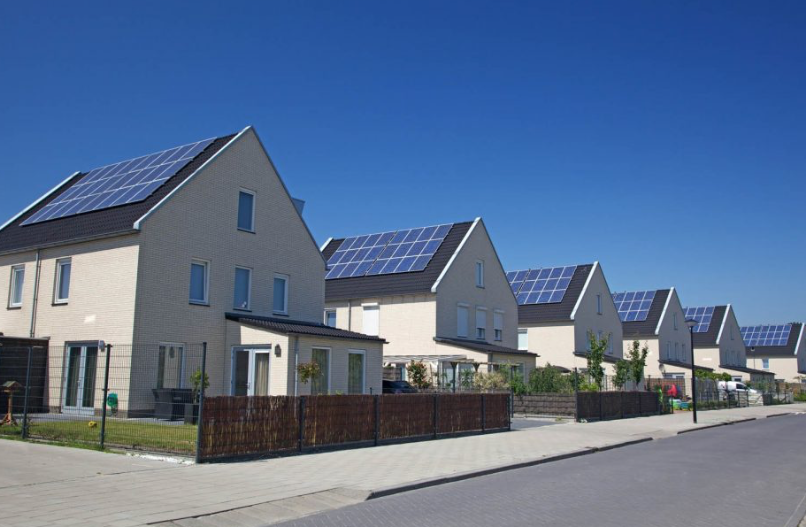
\includegraphics{resid_solar.png}
		}
		\scalebox{0.255}{
			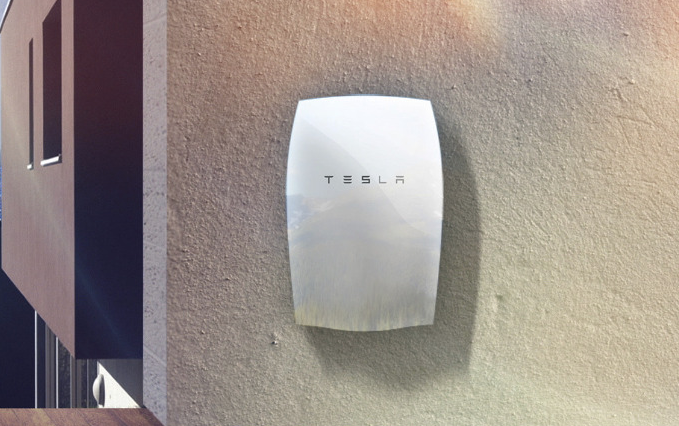
\includegraphics{resid_battery.png}
    		}
	\end{minipage}

\end{frame}

%%=========================================================================================%%
\begin{frame}
	\frametitle{Distributed energy resources in a microgrid}
	\framesubtitle{Optimisation and control}

	\begin{itemize}
		\item  Suppose that:
		\begin{itemize}
			\item  Microgrid has a thin gateway connection to the main grid
			\item  Each household is equipped with rooftop solar panels and a residential battery
		\end{itemize}
		
		\item  Model power imported from/ exported to the main grid as a function of DER in the microgrid
		
		\item  Implement controller to optimise DER in the microgrid
		
		\item  Perform virtual trials (i.e., equation-based simulations using real-world data) to examine:
		\begin{itemize}
			\item  Objective function and process constraints that minimise the cost of power imported from the grid while reducing operational maximum demand
			\item  Effect of electricity tariff structure on the operational load profile
			\item  Savings achieved by optimising at the microgrid level rather than the individual household level
		\end{itemize}
	
	\end{itemize}

\end{frame}

%%=========================================================================================%%
\begin{frame}
	\frametitle{Notation}
	\framesubtitle{Single-period setting}
	
	\begin{tabular}{l l l}
		Let & $m$ & be the number of households in the microgrid\\
		& $n$ & number of time intervals in the prediction and control horizons\\
		& $N$ & number of time intervals in the simulation horizon\\
		& $\delta$ & conversion factor from power (kW) to energy (kWh)\\
		& $\eta$ & one-way battery charge/discharge efficiency\\
		& $\boldsymbol{c}(t)$ & vector of weighting coefficients (e.g., tariffs) for time interval~$t$\\
		& $p_{i}(t)$ & power imported from the grid by household~$i$ during time interval~$t$\footnote{
$p_{i}(t) < 0$ implies power exported to the grid	
}\\
		& $b_{i}(t)$ & battery charge control signal for household~$i$ resolved at time~$t$\footnote{\label{fn:symbol1}
Control signals resolved at time~$t$ apply during time interval~$t\!+\!1$
}\\
		& $d_{i}(t)$ & battery discharge control signal for household~$i$ resolved at time~$t$\textsuperscript{\ref{fn:symbol1}}\\
		& $\el_{i}(t)$ & load generated by household~$i$ forecast at time~$t$\footnote{\label{fn:symbol2}
Control signals set to forecasts produced at time~$t$ are valid for time interval~$t\!+\!1$
}\\
		& $g_{i}(t)$ & power generated by rooftop PV of household~$i$ forecast at time~$t$\textsuperscript{\ref{fn:symbol2}}\\
		& $e_{i}(t)$ & state of charge (SOC) of the battery of household~$i$ at time~$t$\\	
	\end{tabular}
	
\end{frame}

%%=========================================================================================%%
\begin{frame}
	\frametitle{State-space model predictive control (MPC)}
	\framesubtitle{Single-period state-space model}

	\begin{itemize}
		\item  MPC discretises prediction, control and simulation horizons into half-hourly time intervals (i.e., $\delta = 0.50$)
		\item  Suppose that discrete times $t\!-\!1$ and $t$, respectively, translate to clock times $\varsigma$ and $\tau$; then ``at time~$t$'' refers to clock time~$\tau$, and ``during time interval~$t$'' refers to clock time interval $(\varsigma, \tau]$
		\item  State-space model of DER in a microgrid represents power imported from/ exported to the main grid as a function of load, rooftop PV generation, and power charging, or discharged from, the battery
		\begin{IEEEeqnarray*}{rCl}
                	% State-space matrix equation representing DER in a microgrid
                		\underset{\boldsymbol{y}_{i}(t+1)}{
                		\begin{bmatrix*}[c]
    				p_{i}(t\!+\!1)	\\
                			e_{i}(t\!+\!1)
                		\end{bmatrix*}}
                		& = &
                		\underset{A}{
                		\begin{bmatrix*}[c]
                			0	& 0	\\
                			0	& 1
                    	\end{bmatrix*}}
                		\underset{\boldsymbol{x}_{i}(t)}{
                		\begin{bmatrix*}[c]
                			p_{i}(t)	\\
                			e_{i}(t)
                		\end{bmatrix*}}
                		+
                		\underset{B}{
                		\begin{bmatrix*}[c]
    				1			& -1			& 1	& -1	\\
                			\mwmwh\eff	& -\mwmwh/\eff	& 0	& 0	
                 	\end{bmatrix*}}
                		\underset{\boldsymbol{u}_{i}(t)}{
                		\begin{bmatrix*}[c]
                			b_{i}(t)	\\
                			d_{i}(t)	\\
                			\el_{i}(t)	\\
    				g_{i}(t)
                		\end{bmatrix*}}
		\end{IEEEeqnarray*}
		for $i = 1, \ldots, m$ and $t=1, \ldots, N$
	\end{itemize}

\end{frame}

%%=========================================================================================%%
\begin{frame}
	\frametitle{State-space model predictive control (MPC)}
	\framesubtitle{Multi-period prediction and control horizons}

	\begin{itemize}
		\item  Set receding prediction/control horizons to 8 hours (${n=16}$), and let
		\begin{IEEEeqnarray*}{rCl}
			\vv{\boldsymbol{y}}_{i,t+1} & = & \begin{bmatrix*}[c] \boldsymbol{y}_{i}(t\!+\!1)^{T} &\boldsymbol{y}_{i}(t\!+\!2)^{T} & \!\ldots\! & \boldsymbol{y}_{i}(t\!+\!n)^{T} \end{bmatrix*}^{T},\\
			\vv{\boldsymbol{u}}_{i,t} & = & \begin{bmatrix*}[c] \boldsymbol{u}_{i}(t)^{T} &\boldsymbol{u}_{i}(t\!+\!1)^{T} & \!\ldots\! & \boldsymbol{u}_{i}(t\!+\!n\!-\!1)^{T} \end{bmatrix*}^{T}
		\end{IEEEeqnarray*}
		
		\item  Recursively applying the single-period model 
		\begin{equation*}
			\boldsymbol{y}_{i}(t\!+\!1) = A\boldsymbol{x}_{i}(t) + B\boldsymbol{u}_{i}(t)
		\end{equation*}
		over the $n$-period horizon yields
		\begin{equation*}
			\vv{\boldsymbol{y}}_{i,t+1} = K\boldsymbol{x}_{i}(t) + L\vv{\boldsymbol{u}}_{i,t},
		\end{equation*}
		where
		\begin{equation*}
			K =
			\begin{bmatrix*}[c]
			A		\\
			A^{2}	\\
			\vdots	\\
			A^{n}
    			\end{bmatrix*}\;\text{and}\;
			L =
			\begin{bmatrix*}[c]
			B			& 0			& 0		& \ldots			& 0		\\
			AB			& B			& 0		& \ldots			& 0		\\
			\vdots		& \vdots		& \multicolumn{2}{c}{\ddots}	& \vdots	\\
			A^{n\!-\!1}B	& A^{n\!-\!2}B	& \ldots	& AB				& B	
    			\end{bmatrix*}
		\end{equation*}
		for $i = 1, \ldots, m$ and $t=1, \ldots, N$
	
	\end{itemize}
		
\end{frame}

%%=========================================================================================%%
\begin{frame}
	\frametitle{MPC controller}
	\framesubtitle{Multi-period performance index}

	\begin{itemize}
		\item  Performance index is weighted to reflect cost of power imported from the grid
		\item  Define the multi-period performance index as
		\begin{IEEEeqnarray*}{rCl}
				f & = & \left\lVert\sqrts{\Lambda}\big(K\boldsymbol{x}_{i}(t) + L\vv{\boldsymbol{u}}_{i,t}\big)\right\rVert_{2}^{2},
		\end{IEEEeqnarray*}
		where $\Lambda = \operatorname{diag}\big([\boldsymbol{c}(t\!+\!1)^{T}, \boldsymbol{c}(t\!+\!2)^{T}, \ldots, \boldsymbol{c}(t\!+\!n)^{T}]\big)$ is a positive semi-definite diagonal weighting matrix reflecting the electricity tariff structure
		
		\item  Optimisation of performance index is subject to process constraints:
		\begin{itemize}
			\item  Rooftop PV generation and load are set to solar power and demand forecasts %--- virtual trials assume perfect foresight
			\item  One-way battery charge/discharge efficiency%, $\eta = \sqrts{0.88}$
			\item  Charge/discharge rates cannot exceed rated power (continuous) of the battery
			\item  Energy capacity accounts for its decay over the lifetime of the battery
			\item  Upper and lower bounds on SOC restrict battery to partial discharging, which prolongs battery life
			\item  Linear complementarity of battery charge and discharge control signals
		\end{itemize}
		
	\end{itemize}

\end{frame}

%%=========================================================================================%%
\begin{frame}
	\frametitle{MPC controller}
	\framesubtitle{Multi-period mixed integer quadratic programming}

	\begin{itemize}
		\item  Expanding the performance index, dropping the constant terms and imposing process constraints, the quadratic program is written in standard form
		\begin{IEEEeqnarray*}{rCl}
			\underset{\vv{\boldsymbol{u}}_{i,t}}{\operatorname{argmin}} & \quad & \frac{1}{2}\vv{\boldsymbol{u}}_{i,t}^{T}\left(L^{T}\Lambda{L}\right)\vv{\boldsymbol{u}}_{i,t} + \big(K\boldsymbol{x_{i}}(t)\big)^{T}\Lambda{L}\vv{\boldsymbol{u}}_{i,t}	\\
    			\operatorname{subject\ to} & &  \underline{b_{i}} \leq b_{i}(t\!+\!k\!-\!1) \leq \overline{b_{i}},\\
		& & \underline{d_{i}} \leq d_{i}(t\!+\!k\!-\!1) \leq \overline{d_{i}},\\
		& & \underline{e}_{i} \leq e_{i}(t\!+\!k\!-\!1) + {\delta\eta}b_{i}(t\!+\!k\!-\!1) - \frac{\delta}{\eta}d_{i}(t\!+\!k\!-\!1) \leq \overline{e}_{i},\\
		& & b_{i}(t\!+\!k\!-\!1) = 0{\quad\operatorname{or}\quad}d_{i}(t\!+\!k\!-\!1) = 0,\\
		& & k = 1, \ldots, n
		\end{IEEEeqnarray*}
		for $i = 1, \ldots, m$ and $t=1, \ldots, N$
		
		\item  Introducing binary variable to ensure linear complementarity transforms the optimisation into a mixed linear quadratic program (MIQP)
	\end{itemize}

\end{frame}

%%=========================================================================================%%
\begin{frame}
	\frametitle{Optimisation and control}
	\framesubtitle{Mixed integer linear programming}

	\begin{itemize}
		\item  Let $p_{i}(t) \geq 0$ be power imported from the grid by household~$i$ during time interval~$t$, and $q_{i}(t) \geq 0$ power exported to the grid by household~$i$ during time interval~$t$
		
		\item  Power balance equation is given by
		\begin{IEEEeqnarray*}{rCl}
			p_{i}(t\!+\!k) & = & b_{i}(t\!+\!k\!-\!1) - d_{i}(t\!+\!k\!-\!1) +\\
			& & \el_{i}(t\!+\!k\!-\!1) - g_{i}(t\!+\!k\!-\!1)  + q_{i}(t\!+\!k),\\
			& & k = 1, \ldots, n
		\end{IEEEeqnarray*}
		for $i = 1, \ldots, m$ and $t = 1, \ldots, N$
		
		\item  Introduce additional binary variable to ensure linear complementarity of power imported from and power exported to the grid
		
	\end{itemize}

\end{frame}

%%=========================================================================================%%
\begin{frame}
	\frametitle{Optimisation and control}
	\framesubtitle{Mixed integer linear programming}
	
	\begin{IEEEeqnarray*}{rCl}
    		\operatorname{minimise} & \quad & \sum_{k=1}^{n} c(t\!+\!k)p_{i}(t\!+\!k)\\
		\operatorname{subject\ to} & & \underline{b_{i}} \leq b_{i}(t\!+\!k\!-\!1) \leq \overline{b_{i}},\\
		& & \underline{d_{i}} \leq d_{i}(t\!+\!k\!-\!1) \leq \overline{d_{i}},\\
		& & \underline{e}_{i} \leq e_{i}(t\!+\!k\!-\!1) + {\delta\eta}b_{i}(t\!+\!k\!-\!1) - \frac{\delta}{\eta}d_{i}(t\!+\!k\!-\!1) \leq \overline{e}_{i},\\
		& & b_{i}(t\!+\!k\!-\!1) = 0{\quad\operatorname{or}\quad}d_{i}(t\!+\!k\!-\!1) = 0,\\
		& & p_{i}(t\!+\!k) = 0{\quad\operatorname{or}\quad}q_{i}(t\!+\!k) = 0,\\
		& & \hat{\el}_{i}(t\!+\!k) \leq \el_{i}(t\!+\!k\!-\!1) \leq \hat{\el}_{i}(t\!+\!k),\\
		& & \hat{g}_{i}(t\!+\!k) \leq g_{i}(t\!+\!k\!-\!1) \leq \hat{g}_{i}(t\!+\!k),\\
		& & k = 1, \ldots, n\\
		\text{for} & & i = 1, \ldots, m \text{~and~} t = 1, \ldots, N\\
	\end{IEEEeqnarray*}

\end{frame}

%%=========================================================================================%%
\begin{frame}
	\frametitle{Data, variables and parameters}
	\framesubtitle{}

	\begin{itemize}
		\item  Real-world data from Salisbury trial:
		\begin{itemize}
			\item  Actual half-hourly time series of rooftop PV generation and load for 75 households over 16-week simulation horizon (04/02/2017--26/05/2017)
			\item  Assume perfect foresight
			\item  No household has more than 0.5\% of 5,378 half-hourly intervals with missing data --- filled with zeroes
		\end{itemize}
		
		\item  Suppose that each household has installed a Tesla Powerwall 2.0 DC battery:
		\begin{itemize}
			\item  11.5 kWh energy storage capacity --- mid-point assuming decay to 70\% of its original capacity over its lifetime
			\item  5 kW power rating (continuous charge and discharge)
			\item  80\% discharge cycle --- SOC maintained between 10\% and 90\%
			\item  88\% round-trip efficiency when coupled to a solar inverter (i.e., $\eta = \sqrts{0.88}$)
		\end{itemize}
		\item  Power imported from the grid is subject to time-of-day (TOD) tariff (\$/kWh)
			\begin{table}[!h]
			\centering
			{\scriptsize
			\begin{tabular}{c c c c}
				\toprule
				& Off-peak	& Shoulder	& Peak	\\
				&	& 12:00--16:00	& 16:00--21:00	\\
				\midrule
				April--October	& 0.24	& 0.36	& 0.36	\\
				November--March	& 0.24	& 0.36	& 0.48	\\
				\bottomrule
			\end{tabular}
			}
			\end{table}
		while power exported to the grid earns a feed-in tariff of \$0.08/kWh
	
	\end{itemize}

\end{frame}

%%=========================================================================================%%
\begin{frame}
	\frametitle{Virtual trials}
	\framesubtitle{}

	\begin{itemize}
		\item  MPC controller determines battery charge/discharge control signals that minimise cost of power imported from the grid subject to process constraints
		
		\item  Evaluate optimisation algorithms, control techniques and simulation parameters by their effect on:
		\begin{itemize}
			\item  Net cost of electricity for households
			\item  Operational peak demand (i.e., network upgrades)
			\item  Battery charge/discharge cycles (i.e., life of the battery)
			\item  Simulation runtime
		\end{itemize}
		
		\item  Virtual trials compare:
		\begin{itemize}
			\item  No battery energy storage versus Tesla Powerwall 2.0 DC installed
			\item  Single-period (half-hour, tariff independent) versus multi-period (8 hours, TOD tariff) control horizon
			\item  Optimisation at the household level versus the microgrid level\footnote{\scriptsize Microgrid level opitimisation simply aggregates rooftop PV generation, load and energy storage capacity across households in the microgrid for each half-hourly interval
			}
			%\item  Different vectors of weighting coefficients applied over a multi-period control horizon versus weighting based on TOD tariff
			\item  MILP versus MIQP algorithm
		\end{itemize}
	
	\end{itemize}

\end{frame}

%%=========================================================================================%%
\begin{frame}
	\frametitle{Virtual trials}
	\framesubtitle{Empirical research findings}

	\begin{enumerate}
		\item  Battery energy storage reduces net cost of electricity substantially
			\vspace{-0.5em}
			\begin{table}[!h]
			\centering
			{\scriptsize
			\begin{tabular}{l r r r}
				\toprule
				& \multicolumn{1}{c}{Net cost of}	& \multicolumn{1}{c}{Operational peak}	& \multicolumn{1}{c}{Charge/discharge}	\\
				& \multicolumn{1}{c}{	electricity (\$)} 	& \multicolumn{1}{c}{demand (kW)}		&\multicolumn{1}{c}{cycles}	\\
				\midrule
				MIQP, household, single-period, no BESS	& 28,086	& 242.8	& N/A	\\
				MIQP, household, single-period, BESS	& 16,017	& 183.8	& 74.3	\\
				\midrule
				\% change	& -43.0	& -24.3	& N/A	\\
				\bottomrule
			\end{tabular}
			}
			\end{table}
		
		
		\item  Further cost savings are achieved by optimising at the microgrid level relative to the individual household level
			\vspace{0.5em}
			\begin{table}[!h]
			\centering
			{\scriptsize
			\begin{tabular}{l r r r}
				\toprule
				& \multicolumn{1}{c}{Net cost of}	& \multicolumn{1}{c}{Operational peak}	& \multicolumn{1}{c}{Charge/discharge}	\\
				& \multicolumn{1}{c}{	electricity (\$)} 	& \multicolumn{1}{c}{demand (kW)}		&\multicolumn{1}{c}{cycles}	\\
				\midrule
				MIQP, household, single-period		& 16,017	& 183.8	& 74.3	\\
				MIQP, microgrid, single-period		& 11,956	& 242.8	& 82.1	\\
				\midrule
				\% change	& -25.4	& 32.1	& 10.6	\\
				\bottomrule
			\end{tabular}
			}
			\end{table}
			
		\setcounter{enumcount}{\value{enumi}}
	\end{enumerate}

\end{frame}

%%=========================================================================================%%
\begin{frame}
	\frametitle{Virtual trials}
	\framesubtitle{Empirical research findings}

	\begin{enumerate}
		\setcounter{enumi}{\value{enumcount}}		
		\item  Peak operational demand is markedly lower for a multi-period control horizon employing MIQP relative to a single-period control horizon
			\begin{table}[!h]
			\centering
			{\scriptsize
			\begin{tabular}{l r r r}
				\toprule
				& \multicolumn{1}{c}{Net cost of}	& \multicolumn{1}{c}{Operational peak}	& \multicolumn{1}{c}{Charge/discharge}	\\
				& \multicolumn{1}{c}{	electricity (\$)} 	& \multicolumn{1}{c}{demand (kW)}		&\multicolumn{1}{c}{cycles}	\\
				\midrule
				MIQP, microgrid, single-period		& 11,956	& 242.8	& 82.1	\\
				MIQP, microgrid, multi-period		& 12,285	& 152.7	& 89.4	\\
				\midrule
				\% change	& 2.7		& -37.1	& 8.8		\\
				\bottomrule
			\end{tabular}
			}
			\end{table}
		
		\item  Differences between MIQP and MILP algorithms for a single-period control horizon is marginal
			\begin{table}
			\centering
			{\scriptsize
			\begin{tabular}{l r r r}
				\toprule
				& \multicolumn{1}{c}{Net cost of}	& \multicolumn{1}{c}{Operational peak}	& \multicolumn{1}{c}{Charge/discharge}	\\
				& \multicolumn{1}{c}{	electricity (\$)} 	& \multicolumn{1}{c}{demand (kW)}		&\multicolumn{1}{c}{cycles}	\\
				\midrule
				MIQP, microgrid, single-period		& 11,956	& 242.8	& 82.1	\\
				MILP, microgrid, single-period		& 11,997	& 242.8	& 82.1	\\
				\midrule
				\% change	& 0.3		& 0.0		& 0.0		\\
				\bottomrule
			\end{tabular}
			}
			\end{table}
		
		\setcounter{enumcount}{\value{enumi}}	
	\end{enumerate}

\end{frame}

%%=========================================================================================%%
\begin{frame}
	\frametitle{Virtual trials}
	\framesubtitle{Empirical research findings}

	\begin{enumerate}
		\setcounter{enumi}{\value{enumcount}}
		\item  Operational peak demand for a multi-period control horizon employing MIQP is a fraction of that employing MILP\footnote{\scriptsize QP penalises large power imports from the grid during a given time interval disproportionately more heavily than small imports, while LP penalises large power imports from the grid during a given time interval proportionately equally as small imports
		}
			\begin{table}
			\centering
			{\scriptsize
			\begin{tabular}{l r r r}
				\toprule
				& \multicolumn{1}{c}{Net cost of}	& \multicolumn{1}{c}{Operational peak}	& \multicolumn{1}{c}{Charge/discharge}	\\
				& \multicolumn{1}{c}{	electricity (\$)} 	& \multicolumn{1}{c}{demand (kW)}		&\multicolumn{1}{c}{cycles}	\\
				\midrule
				MILP, microgrid, multi-period		& 12,748	& 434.4	& 83.6	\\
				MIQP, microgrid, multi-period		& 12,285	& 152.7	& 89.4	\\
				\midrule
				\% change	& -3.6		& -64.9		& 7.0		\\
				\bottomrule
			\end{tabular}
			}
			\end{table}
		
		\item  MILP (48 min 10 sec) solves faster than MIQP (2 hr 11 min 29 sec) on an iMac with 2.7 GHz processor and 8 GB memory when optimising DER in a microgrid at the household level over a multi-period control horizon\footnote{\scriptsize MPC controller is coded in \textsc{MATLAB} and invokes solvers \texttt{cplexmilp()} and \texttt{cplexmilp()} from the CPLEX for \textsc{MATLAB} Toolbox
		}
	
	\end{enumerate}

\end{frame}

%%=========================================================================================%%
\begin{frame}
	\frametitle{Actual DER management}
	\framesubtitle{Salisbury trial}

	\begin{table}
	\centering
	\begin{tabular}{l r @{ } l}
		\toprule
		\multicolumn{3}{c}{\textit{75 households in 16-week Salisbury trial}}	\\
		\multicolumn{3}{c}{\textit{from 04/02/2017 to 26/05/2017}}	\\
		\midrule
		Consumption				& 177,527&kWh	\\
		Rooftop PV generation 		& 152,310&kWh	\\
		Energy charging battery		& 45,627&kWh		\\
		Energy discharge from battery	& 42,064&kWh		\\
		Operational peak demand		& 217.7&kW		\\
		Energy imported from the grid	& 79,020&kWh		\\
		Energy exported to the grid	& 49,945&kWh		\\
		Net cost of electricity			& \$19,316&		\\
		\bottomrule
	\end{tabular}
	\end{table}

\end{frame}

%%=========================================================================================%%
\begin{frame}
	\frametitle{Other applied mathematics research on clean energy}
	\framesubtitle{Dependable supply of wind power with battery energy storage}
	
	\begin{minipage}{0.55\linewidth}
		\begin{itemize}
			\item  Tilt Renewables has announced that it will connect a solar farm (44MW) and utility-scale battery (21MW/26MWh) to its Snowtown wind farm (369MW) in the mid-north of South Australia
		
			\item  Collaboration with Tilt Renewables is applying optimisation and control techniques to firm-up wind power dispatch using battery energy storage
			
			\item  Conjecture that if wind farms were to dependably supply power scheduled during pre-dispatch, then wholesale electricity prices would be less volatile and, on average, lower 
	
		\end{itemize}
	\end{minipage}%
	\begin{minipage}{0.45\linewidth}
		\scalebox{0.261}{
			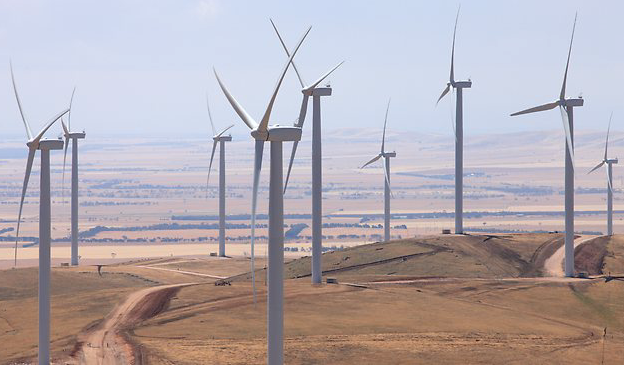
\includegraphics{wind_farm.png}
		}
		\scalebox{0.164}{
			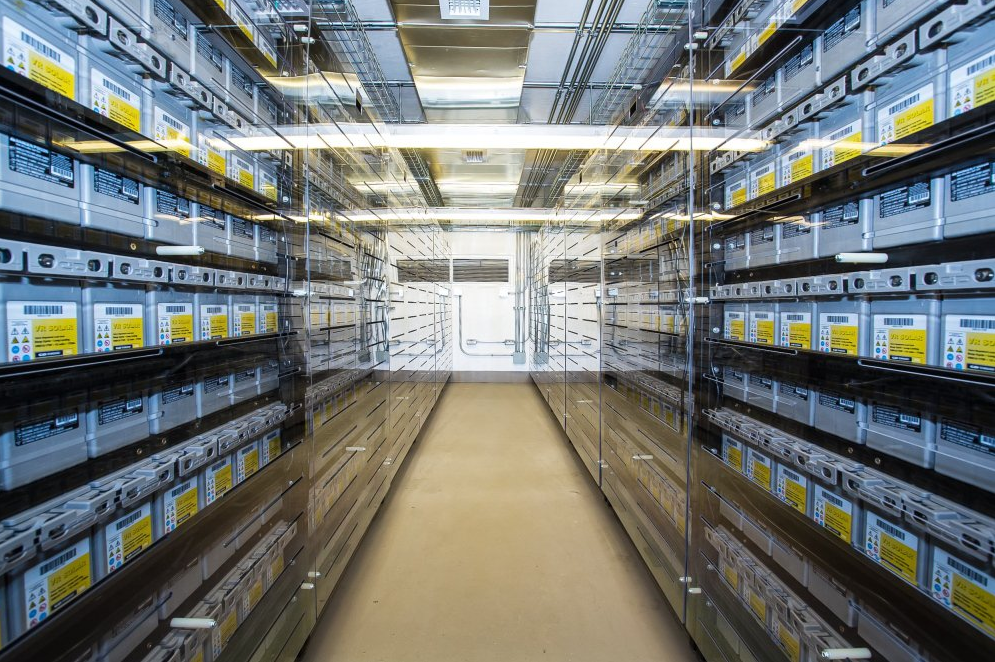
\includegraphics{utility_battery.png}
    		}
	\end{minipage}

	
\end{frame}


%%=========================================================================================%%
\end{document}

%%=========================================================================================%%
%%=========================================================================================%%
\begin{frame}
	\frametitle{<frame title>}
	\subframetitle{<subframe title>}

	<introductory statement>
	\begin{itemize}
		\item  <first item>
		\item  <more items>
	\end{itemize}
	
	\begin{figure}[!h]
	\centering
    	\label{fig:<label>}
	\scalebox{0.80}{
		\includegraphics{<file.pdf>}
		\input{<file>}
	}
	\end{figure}
	

\note[item]{
<notes>
}
\end{frame}

%%=========================================================================================%%


